\documentclass[openany]{swufethesis}

\usepackage{booktabs}
\usepackage{hyperref}

\addbibresource{sample.bib}

\swufesetup{
  date = 2021-01-04,
  title = 西南财经大学学位论文\LaTeX 模板示例文档,
  author = 韭菜盒子想毕业,
  school = 经济信息工程学院,
  discipline = 计算机科学与技术(金融信息化方向),
  student-id = 41799999,
  supervisor = XX教授,
  degree = bachelor,
}

\begin{document}
\maketitle % 封面
\statement % 版权申明

\begin{abstract}{毕业论文, 毕业设计, 西南财经大学}
  摘要内容应概括地反映出本论文的主要内容,主要说明本论文的研究目的、
  内容、方法、成果和结论。语言力求精练、准确,摘要字数300字左右。

  关键词是供检索用的主题词条。摘要与关键词应在同一页。关键词一般3--5个。
\end{abstract}

\begin{abstract*}{Dissertation, Graduation project, Swufe}
  An abstract of a dissertation should reflect the main content in a general way,
  mainly stating the research objective, content, methodology, results and conclusions
  of the dissertation. The language should be concise and accurate, and the abstract
  should be about 250--400 words.

  Keywords are subject entries for indexing. The abstract and keywords should be
  on the same page. And an abstract generally contains 3--5 keywords.
\end{abstract*}

\tableofcontents

\mainmatter % \mainmatter会重置页码样式为阿拉伯数字,并使\chapter被编号
\chapter{毕业论文的撰写规范}
本科生毕业论文写作是反映学生毕业论文工作成效的重要途经,是考核学生
掌握和运用所学基础理论、基本知识、基本技能从事科学研究和解决实际问题能
力的有效手段。掌握撰写毕业论文的基本能力是本科人才培养中的一个十分重要
的环节。
\section{论文题目}
论文题目应以简短、明确的词语恰当概括论文的核心内容,避免使用不常见
的缩略词、缩写字。中文题目一般不宜超过24个字,必要时可增加副标题。外
文题目一般不宜超过12个实词。

\section{摘要与关键词}
摘要内容应概括地反映出本论文的主要内容,主要说明本论文的研究目的、
内容、方法、成果和结论。语言力求精练、准确,摘要字数300字左右。

关键词是供检索用的主题词条。摘要与关键词应在同一页。关键词一般3--5个。

英文摘要内容与中文摘要相同,以250--400个实词为宜。

\section{正文的结构}
正文是毕业论文的主体和核心部分,不同学科专业和不同的选题可以有不
同的写作方式。非外语专业的毕业论文应用中文撰写,如用英文撰写,请附上中
文的全文翻译。正文一般包括以下几个方面:引言或背景、主体和结论。

\section{名词术语}
科学技术名词术语尽量采用全国自然科学名词审定委员会公布的规范词
或国家标准、部标准中规定的名称,尚未统一规定或叫法有争议的名词术语,可
采用惯用的名称。

特定含义的名词术语或新名词、以及使用外文缩写代替某一名词术语时,
首次出现时应在括号内注明其含义。

外国人名一般采用英文原名,可不译成中文,英文人名按姓前名后的原
则书写。一般很熟知的外国人名(如牛顿、爱因斯坦、达尔文、马克思等)可按通
常标准译法写译名。

\section{注释}
毕业论文中有个别名词或情况需要解释时,可加注说明。\footnote{注释采用脚注,每
  页独立编号,即每页都从1开始编码,编号用1、2、3、……,文中编号用上标。}

\chapter{参考文献的标注}
参考文献是毕业论文不可缺少的组成部分,它反映毕业论文的取材来源、材
料的广博程度和材料的可靠程度,也是作者对他人知识成果的承认和尊重。

一个英文文献\cite{dirac}提出了,一个中文文献\cite{蔡敏2006--}提出了balabala。

\begin{table}[htb]
  \caption{表格示例}
  \centering
  \begin{tabular}{lrrrr}
    \toprule
    项目 & 指标  \\
    \midrule
    A    & 1.7   \\
    B    & 1.2   \\
    C    & -12.6 \\
    \bottomrule
  \end{tabular}
\end{table}

\begin{figure}[htb]
  \centering
  
\includegraphics[width=0.4\textwidth]{figures/example-image-a.pdf}
  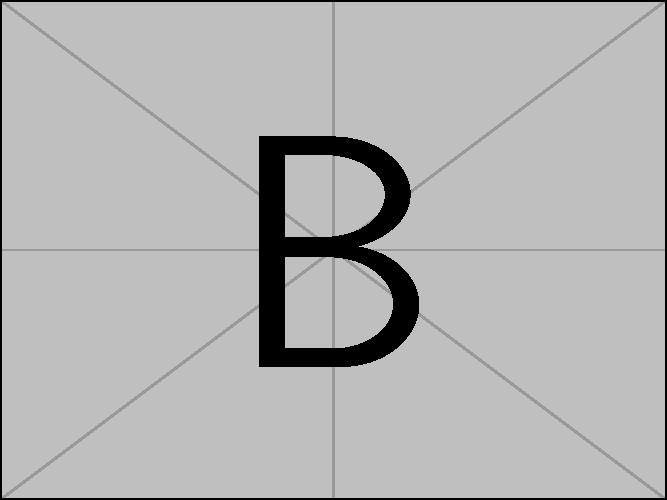
\includegraphics[width=0.4\textwidth]{figures/example-image-b.pdf}
  \caption{图片示例}
\end{figure}

\printbibliography
\appendix
\chapter{补充内容}
如果有不宜放在正文中的重要支撑材料,可编入毕业论文的附录中。包括某
些重要的原始数据、详细数学推导、程序全文及其说明、复杂的图表、设计图纸
等一系列需要补充提供的说明材料。附录的篇幅不宜太多,一般不超过正文。
\begin{verbatim}
Some mono font
\end{verbatim}
\begin{acknowledgments}
  谢辞应以简短的文字对课题研究与论文撰写过程中曾直接给予帮助的人员
  (例如指导教师、答疑教师及其他人员)表示对自己的谢意,这不仅是一种礼
  貌,也是对他人劳动的尊重,是治学者应当遵循的学术规范。内容限一页。
\end{acknowledgments}

\end{document}
